\documentclass[1p]{elsarticle_modified}
%\bibliographystyle{elsarticle-num}

%\usepackage[colorlinks]{hyperref}
%\usepackage{abbrmath_seonhwa} %\Abb, \Ascr, \Acal ,\Abf, \Afrak
\usepackage{amsfonts}
\usepackage{amssymb}
\usepackage{amsmath}
\usepackage{amsthm}
\usepackage{scalefnt}
\usepackage{amsbsy}
\usepackage{kotex}
\usepackage{caption}
\usepackage{subfig}
\usepackage{color}
\usepackage{graphicx}
\usepackage{xcolor} %% white, black, red, green, blue, cyan, magenta, yellow
\usepackage{float}
\usepackage{setspace}
\usepackage{hyperref}

\usepackage{tikz}
\usetikzlibrary{arrows}

\usepackage{multirow}
\usepackage{array} % fixed length table
\usepackage{hhline}

%%%%%%%%%%%%%%%%%%%%%
\makeatletter
\renewcommand*\env@matrix[1][\arraystretch]{%
	\edef\arraystretch{#1}%
	\hskip -\arraycolsep
	\let\@ifnextchar\new@ifnextchar
	\array{*\c@MaxMatrixCols c}}
\makeatother %https://tex.stackexchange.com/questions/14071/how-can-i-increase-the-line-spacing-in-a-matrix
%%%%%%%%%%%%%%%

\usepackage[normalem]{ulem}

\newcommand{\msout}[1]{\ifmmode\text{\sout{\ensuremath{#1}}}\else\sout{#1}\fi}
%SOURCE: \msout is \stkout macro in https://tex.stackexchange.com/questions/20609/strikeout-in-math-mode

\newcommand{\cancel}[1]{
	\ifmmode
	{\color{red}\msout{#1}}
	\else
	{\color{red}\sout{#1}}
	\fi
}

\newcommand{\add}[1]{
	{\color{blue}\uwave{#1}}
}

\newcommand{\replace}[2]{
	\ifmmode
	{\color{red}\msout{#1}}{\color{blue}\uwave{#2}}
	\else
	{\color{red}\sout{#1}}{\color{blue}\uwave{#2}}
	\fi
}

\newcommand{\Sol}{\mathcal{S}} %segment
\newcommand{\D}{D} %diagram
\newcommand{\A}{\mathcal{A}} %arc


%%%%%%%%%%%%%%%%%%%%%%%%%%%%%5 test

\def\sl{\operatorname{\textup{SL}}(2,\Cbb)}
\def\psl{\operatorname{\textup{PSL}}(2,\Cbb)}
\def\quan{\mkern 1mu \triangleright \mkern 1mu}

\theoremstyle{definition}
\newtheorem{thm}{Theorem}[section]
\newtheorem{prop}[thm]{Proposition}
\newtheorem{lem}[thm]{Lemma}
\newtheorem{ques}[thm]{Question}
\newtheorem{cor}[thm]{Corollary}
\newtheorem{defn}[thm]{Definition}
\newtheorem{exam}[thm]{Example}
\newtheorem{rmk}[thm]{Remark}
\newtheorem{alg}[thm]{Algorithm}

\newcommand{\I}{\sqrt{-1}}
\begin{document}

%\begin{frontmatter}
%
%\title{Boundary parabolic representations of knots up to 8 crossings}
%
%%% Group authors per affiliation:
%\author{Yunhi Cho} 
%\address{Department of Mathematics, University of Seoul, Seoul, Korea}
%\ead{yhcho@uos.ac.kr}
%
%
%\author{Seonhwa Kim} %\fnref{s_kim}}
%\address{Center for Geometry and Physics, Institute for Basic Science, Pohang, 37673, Korea}
%\ead{ryeona17@ibs.re.kr}
%
%\author{Hyuk Kim}
%\address{Department of Mathematical Sciences, Seoul National University, Seoul 08826, Korea}
%\ead{hyukkim@snu.ac.kr}
%
%\author{Seokbeom Yoon}
%\address{Department of Mathematical Sciences, Seoul National University, Seoul, 08826,  Korea}
%\ead{sbyoon15@snu.ac.kr}
%
%\begin{abstract}
%We find all boundary parabolic representation of knots up to 8 crossings.
%
%\end{abstract}
%\begin{keyword}
%    \MSC[2010] 57M25 
%\end{keyword}
%
%\end{frontmatter}

%\linenumbers
%\tableofcontents
%
\newcommand\colored[1]{\textcolor{white}{\rule[-0.35ex]{0.8em}{1.4ex}}\kern-0.8em\color{red} #1}%
%\newcommand\colored[1]{\textcolor{white}{ #1}\kern-2.17ex	\textcolor{white}{ #1}\kern-1.81ex	\textcolor{white}{ #1}\kern-2.15ex\color{red}#1	}

{\Large $\underline{11a_{124}~(K11a_{124})}$}

\setlength{\tabcolsep}{10pt}
\renewcommand{\arraystretch}{1.6}
\vspace{1cm}\begin{tabular}{m{100pt}>{\centering\arraybackslash}m{274pt}}
\multirow{5}{120pt}{
	\centering
	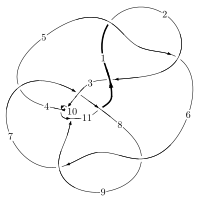
\includegraphics[width=112pt]{../../../GIT/diagram.site/Diagrams/png/373_11a_124.png}\\
\ \ \ A knot diagram\footnotemark}&
\allowdisplaybreaks
\textbf{Linearized knot diagam} \\
\cline{2-2}
 &
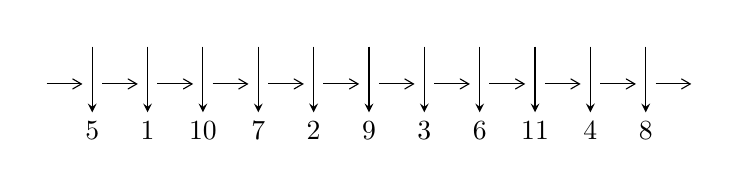
\begin{tikzpicture}[x=20pt, y=17pt]
	% nodes
	\node (C0) at (0, 0) {};
	\node (C1) at (1, 0) {};
	\node (C1U) at (1, +1) {};
	\node (C1D) at (1, -1) {5};

	\node (C2) at (2, 0) {};
	\node (C2U) at (2, +1) {};
	\node (C2D) at (2, -1) {1};

	\node (C3) at (3, 0) {};
	\node (C3U) at (3, +1) {};
	\node (C3D) at (3, -1) {10};

	\node (C4) at (4, 0) {};
	\node (C4U) at (4, +1) {};
	\node (C4D) at (4, -1) {7};

	\node (C5) at (5, 0) {};
	\node (C5U) at (5, +1) {};
	\node (C5D) at (5, -1) {2};

	\node (C6) at (6, 0) {};
	\node (C6U) at (6, +1) {};
	\node (C6D) at (6, -1) {9};

	\node (C7) at (7, 0) {};
	\node (C7U) at (7, +1) {};
	\node (C7D) at (7, -1) {3};

	\node (C8) at (8, 0) {};
	\node (C8U) at (8, +1) {};
	\node (C8D) at (8, -1) {6};

	\node (C9) at (9, 0) {};
	\node (C9U) at (9, +1) {};
	\node (C9D) at (9, -1) {11};

	\node (C10) at (10, 0) {};
	\node (C10U) at (10, +1) {};
	\node (C10D) at (10, -1) {4};

	\node (C11) at (11, 0) {};
	\node (C11U) at (11, +1) {};
	\node (C11D) at (11, -1) {8};
	\node (C12) at (12, 0) {};

	% arrows
	\draw[->,>={angle 60}]
	(C0) edge (C1) (C1) edge (C2) (C2) edge (C3) (C3) edge (C4) (C4) edge (C5) (C5) edge (C6) (C6) edge (C7) (C7) edge (C8) (C8) edge (C9) (C9) edge (C10) (C10) edge (C11) (C11) edge (C12) ;	\draw[->,>=stealth]
	(C1U) edge (C1D) (C2U) edge (C2D) (C3U) edge (C3D) (C4U) edge (C4D) (C5U) edge (C5D) (C6U) edge (C6D) (C7U) edge (C7D) (C8U) edge (C8D) (C9U) edge (C9D) (C10U) edge (C10D) (C11U) edge (C11D) ;
	\end{tikzpicture} \\
\hhline{~~} \\& 
\textbf{Solving Sequence} \\ \cline{2-2} 
 &
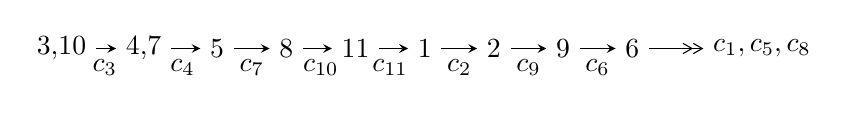
\begin{tikzpicture}[x=25pt, y=7pt]
	% node
	\node (A0) at (-1/8, 0) {3,10};
	\node (A1) at (17/16, 0) {4,7};
	\node (A2) at (17/8, 0) {5};
	\node (A3) at (25/8, 0) {8};
	\node (A4) at (33/8, 0) {11};
	\node (A5) at (41/8, 0) {1};
	\node (A6) at (49/8, 0) {2};
	\node (A7) at (57/8, 0) {9};
	\node (A8) at (65/8, 0) {6};
	\node (C1) at (1/2, -1) {$c_{3}$};
	\node (C2) at (13/8, -1) {$c_{4}$};
	\node (C3) at (21/8, -1) {$c_{7}$};
	\node (C4) at (29/8, -1) {$c_{10}$};
	\node (C5) at (37/8, -1) {$c_{11}$};
	\node (C6) at (45/8, -1) {$c_{2}$};
	\node (C7) at (53/8, -1) {$c_{9}$};
	\node (C8) at (61/8, -1) {$c_{6}$};
	\node (A9) at (10, 0) {$c_{1},c_{5},c_{8}$};

	% edge
	\draw[->,>=stealth]	
	(A0) edge (A1) (A1) edge (A2) (A2) edge (A3) (A3) edge (A4) (A4) edge (A5) (A5) edge (A6) (A6) edge (A7) (A7) edge (A8) ;
	\draw[->>,>={angle 60}]	
	(A8) edge (A9);
\end{tikzpicture} \\ 

\end{tabular} \\

\footnotetext{
The image of knot diagram is generated by the software ``\textbf{Draw programme}" developed by Andrew Bartholomew(\url{http://www.layer8.co.uk/maths/draw/index.htm\#Running-draw}), where we modified some parts for our purpose(\url{https://github.com/CATsTAILs/LinksPainter}).
}\phantom \\ \newline 
\centering \textbf{Ideals for irreducible components\footnotemark of $X_{\text{par}}$} 
 
\begin{align*}
I^u_{1}&=\langle 
u^{17}-2 u^{16}+\cdots+2 b-1,\;8 u^{18}- u^{17}+\cdots+8 a+1,\;u^{19}- u^{18}+\cdots+2 u+1\rangle \\
I^u_{2}&=\langle 
-3.29428\times10^{43} u^{59}-7.32537\times10^{43} u^{58}+\cdots+3.61424\times10^{43} b-3.73726\times10^{43},\\
\phantom{I^u_{2}}&\phantom{= \langle  }-1.15786\times10^{44} u^{59}-2.56717\times10^{44} u^{58}+\cdots+3.61424\times10^{43} a-1.16229\times10^{44},\;u^{60}+3 u^{59}+\cdots+2 u+1\rangle \\
I^u_{3}&=\langle 
b,\;2 a-2 u+3,\;u^2- u-1\rangle \\
\\
\end{align*}
\raggedright * 3 irreducible components of $\dim_{\mathbb{C}}=0$, with total 81 representations.\\
\footnotetext{All coefficients of polynomials are rational numbers. But the coefficients are sometimes approximated in decimal forms when there is not enough margin.}
\newpage
\renewcommand{\arraystretch}{1}
\centering \section*{I. $I^u_{1}= \langle u^{17}-2 u^{16}+\cdots+2 b-1,\;8 u^{18}- u^{17}+\cdots+8 a+1,\;u^{19}- u^{18}+\cdots+2 u+1 \rangle$}
\flushleft \textbf{(i) Arc colorings}\\
\begin{tabular}{m{7pt} m{180pt} m{7pt} m{180pt} }
\flushright $a_{3}=$&$\begin{pmatrix}1\\0\end{pmatrix}$ \\
\flushright $a_{10}=$&$\begin{pmatrix}0\\u\end{pmatrix}$ \\
\flushright $a_{4}=$&$\begin{pmatrix}1\\u^2\end{pmatrix}$ \\
\flushright $a_{7}=$&$\begin{pmatrix}- u^{18}+\frac{1}{8} u^{17}+\cdots+\frac{29}{8} u-\frac{1}{8}\\-\frac{1}{2} u^{17}+u^{16}+\cdots+\frac{5}{2} u+\frac{1}{2}\end{pmatrix}$ \\
\flushright $a_{5}=$&$\begin{pmatrix}0.812500 u^{18}-0.312500 u^{17}+\cdots-2.75000 u+0.687500\\u^3- u\end{pmatrix}$ \\
\flushright $a_{8}=$&$\begin{pmatrix}- u^{18}+\frac{5}{8} u^{17}+\cdots+\frac{9}{8} u-\frac{5}{8}\\-\frac{1}{2} u^{17}+u^{16}+\cdots+\frac{5}{2} u+\frac{1}{2}\end{pmatrix}$ \\
\flushright $a_{11}=$&$\begin{pmatrix}- u\\- u^3+u\end{pmatrix}$ \\
\flushright $a_{1}=$&$\begin{pmatrix}\frac{13}{16} u^{18}-\frac{5}{16} u^{17}+\cdots-\frac{11}{4} u-\frac{5}{16}\\- u^2\end{pmatrix}$ \\
\flushright $a_{2}=$&$\begin{pmatrix}\frac{5}{16} u^{18}-\frac{1}{8} u^{17}+\cdots-\frac{29}{16} u+\frac{1}{2}\\- u^4\end{pmatrix}$ \\
\flushright $a_{9}=$&$\begin{pmatrix}u^3\\u^5- u^3+u\end{pmatrix}$ \\
\flushright $a_{6}=$&$\begin{pmatrix}- u^{18}+\frac{3}{8} u^{17}+\cdots+\frac{23}{8} u-\frac{3}{8}\\u^5- u^3+u\end{pmatrix}$\\ \flushright $a_{6}=$&$\begin{pmatrix}- u^{18}+\frac{3}{8} u^{17}+\cdots+\frac{23}{8} u-\frac{3}{8}\\u^5- u^3+u\end{pmatrix}$\\&\end{tabular}
\flushleft \textbf{(ii) Obstruction class $= -1$}\\~\\
\flushleft \textbf{(iii) Cusp Shapes $= \frac{5}{8} u^{18}+\frac{15}{16} u^{17}+\cdots-\frac{147}{16} u-\frac{275}{16}$}\\~\\
\newpage\renewcommand{\arraystretch}{1}
\flushleft \textbf{(iv) u-Polynomials at the component}\newline \\
\begin{tabular}{m{50pt}|m{274pt}}
Crossings & \hspace{64pt}u-Polynomials at each crossing \\
\hline $$\begin{aligned}c_{1},c_{3},c_{5}\\c_{10}\end{aligned}$$&$\begin{aligned}
&u^{19}- u^{18}+\cdots+2 u+1
\end{aligned}$\\
\hline $$\begin{aligned}c_{2},c_{9}\end{aligned}$$&$\begin{aligned}
&u^{19}+11 u^{18}+\cdots+10 u+1
\end{aligned}$\\
\hline $$\begin{aligned}c_{4},c_{11}\end{aligned}$$&$\begin{aligned}
&4(4 u^{19}-6 u^{18}+\cdots+u+1)
\end{aligned}$\\
\hline $$\begin{aligned}c_{6},c_{8}\end{aligned}$$&$\begin{aligned}
&u^{19}+u^{18}+\cdots+72 u+16
\end{aligned}$\\
\hline $$\begin{aligned}c_{7}\end{aligned}$$&$\begin{aligned}
&u^{19}+5 u^{18}+\cdots+576 u+64
\end{aligned}$\\
\hline
\end{tabular}\\~\\
\newpage\renewcommand{\arraystretch}{1}
\flushleft \textbf{(v) Riley Polynomials at the component}\newline \\
\begin{tabular}{m{50pt}|m{274pt}}
Crossings & \hspace{64pt}Riley Polynomials at each crossing \\
\hline $$\begin{aligned}c_{1},c_{3},c_{5}\\c_{10}\end{aligned}$$&$\begin{aligned}
&y^{19}-11 y^{18}+\cdots+10 y-1
\end{aligned}$\\
\hline $$\begin{aligned}c_{2},c_{9}\end{aligned}$$&$\begin{aligned}
&y^{19}-3 y^{18}+\cdots+6 y-1
\end{aligned}$\\
\hline $$\begin{aligned}c_{4},c_{11}\end{aligned}$$&$\begin{aligned}
&16(16 y^{19}-44 y^{18}+\cdots+27 y-1)
\end{aligned}$\\
\hline $$\begin{aligned}c_{6},c_{8}\end{aligned}$$&$\begin{aligned}
&y^{19}-11 y^{18}+\cdots+5152 y-256
\end{aligned}$\\
\hline $$\begin{aligned}c_{7}\end{aligned}$$&$\begin{aligned}
&y^{19}+3 y^{18}+\cdots+84480 y-4096
\end{aligned}$\\
\hline
\end{tabular}\\~\\
\newpage\flushleft \textbf{(vi) Complex Volumes and Cusp Shapes}
$$\begin{array}{c|c|c}  
\text{Solutions to }I^u_{1}& \I (\text{vol} + \sqrt{-1}CS) & \text{Cusp shape}\\
 \hline 
\begin{aligned}
u &= \phantom{-}0.419051 + 0.893130 I \\
a &= -0.135730 - 0.103762 I \\
b &= -0.724967 + 1.151790 I\end{aligned}
 & \phantom{-}2.04820 + 6.16450 I & -8.26103 - 3.38099 I \\ \hline\begin{aligned}
u &= \phantom{-}0.419051 - 0.893130 I \\
a &= -0.135730 + 0.103762 I \\
b &= -0.724967 - 1.151790 I\end{aligned}
 & \phantom{-}2.04820 - 6.16450 I & -8.26103 + 3.38099 I \\ \hline\begin{aligned}
u &= \phantom{-}0.899345 + 0.246437 I \\
a &= \phantom{-}2.14777 - 1.01558 I \\
b &= \phantom{-}1.204930 + 0.354128 I\end{aligned}
 & -3.77143 - 0.86442 I & -19.7475 + 1.3057 I \\ \hline\begin{aligned}
u &= \phantom{-}0.899345 - 0.246437 I \\
a &= \phantom{-}2.14777 + 1.01558 I \\
b &= \phantom{-}1.204930 - 0.354128 I\end{aligned}
 & -3.77143 + 0.86442 I & -19.7475 - 1.3057 I \\ \hline\begin{aligned}
u &= -1.003450 + 0.392686 I \\
a &= -1.58170 + 0.42470 I \\
b &= -0.13937 + 1.76374 I\end{aligned}
 & -5.55704 + 4.23947 I & -20.3915 - 6.1738 I \\ \hline\begin{aligned}
u &= -1.003450 - 0.392686 I \\
a &= -1.58170 - 0.42470 I \\
b &= -0.13937 - 1.76374 I\end{aligned}
 & -5.55704 - 4.23947 I & -20.3915 + 6.1738 I \\ \hline\begin{aligned}
u &= \phantom{-}0.552607 + 0.734353 I \\
a &= -0.356653 + 0.052498 I \\
b &= \phantom{-}0.56635 - 1.31894 I\end{aligned}
 & \phantom{-}4.59036 + 0.49883 I & -5.13235 + 1.11737 I \\ \hline\begin{aligned}
u &= \phantom{-}0.552607 - 0.734353 I \\
a &= -0.356653 - 0.052498 I \\
b &= \phantom{-}0.56635 + 1.31894 I\end{aligned}
 & \phantom{-}4.59036 - 0.49883 I & -5.13235 - 1.11737 I \\ \hline\begin{aligned}
u &= \phantom{-}1.034010 + 0.500803 I \\
a &= -0.92474 + 1.69869 I \\
b &= -1.81071 + 0.75880 I\end{aligned}
 & -3.99870 - 8.26948 I & -17.0118 + 10.4497 I \\ \hline\begin{aligned}
u &= \phantom{-}1.034010 - 0.500803 I \\
a &= -0.92474 - 1.69869 I \\
b &= -1.81071 - 0.75880 I\end{aligned}
 & -3.99870 + 8.26948 I & -17.0118 - 10.4497 I\\
 \hline 
 \end{array}$$\newpage$$\begin{array}{c|c|c}  
\text{Solutions to }I^u_{1}& \I (\text{vol} + \sqrt{-1}CS) & \text{Cusp shape}\\
 \hline 
\begin{aligned}
u &= -1.047050 + 0.609446 I \\
a &= \phantom{-}2.13795 + 0.40305 I \\
b &= \phantom{-}1.14750 - 1.52008 I\end{aligned}
 & \phantom{-}1.58848 + 10.77560 I & -11.1069 - 9.6699 I \\ \hline\begin{aligned}
u &= -1.047050 - 0.609446 I \\
a &= \phantom{-}2.13795 - 0.40305 I \\
b &= \phantom{-}1.14750 + 1.52008 I\end{aligned}
 & \phantom{-}1.58848 - 10.77560 I & -11.1069 + 9.6699 I \\ \hline\begin{aligned}
u &= -1.136920 + 0.651601 I \\
a &= -1.99873 - 0.44428 I \\
b &= -1.05260 + 1.28107 I\end{aligned}
 & -2.2580 + 17.5240 I & -13.4299 - 10.5127 I \\ \hline\begin{aligned}
u &= -1.136920 - 0.651601 I \\
a &= -1.99873 + 0.44428 I \\
b &= -1.05260 - 1.28107 I\end{aligned}
 & -2.2580 - 17.5240 I & -13.4299 + 10.5127 I \\ \hline\begin{aligned}
u &= \phantom{-}1.36120\phantom{ +0.000000I} \\
a &= -0.900530\phantom{ +0.000000I} \\
b &= -0.770557\phantom{ +0.000000I}\end{aligned}
 & -10.4347\phantom{ +0.000000I} & -25.7620\phantom{ +0.000000I} \\ \hline\begin{aligned}
u &= -0.459746 + 0.391888 I \\
a &= -0.822946 - 0.928476 I \\
b &= -0.928594 + 0.046627 I\end{aligned}
 & -0.672184 - 0.228526 I & -10.04556 + 0.04203 I \\ \hline\begin{aligned}
u &= -0.459746 - 0.391888 I \\
a &= -0.822946 + 0.928476 I \\
b &= -0.928594 - 0.046627 I\end{aligned}
 & -0.672184 + 0.228526 I & -10.04556 - 0.04203 I \\ \hline\begin{aligned}
u &= -0.460389\phantom{ +0.000000I} \\
a &= -0.746543\phantom{ +0.000000I} \\
b &= -0.475486\phantom{ +0.000000I}\end{aligned}
 & -0.745623\phantom{ +0.000000I} & -13.0540\phantom{ +0.000000I} \\ \hline\begin{aligned}
u &= \phantom{-}1.58350\phantom{ +0.000000I} \\
a &= -0.283362\phantom{ +0.000000I} \\
b &= -0.279027\phantom{ +0.000000I}\end{aligned}
 & -10.5925\phantom{ +0.000000I} & -69.4310\phantom{ +0.000000I}\\
 \hline 
 \end{array}$$\newpage\newpage\renewcommand{\arraystretch}{1}
\centering \section*{II. $I^u_{2}= \langle -3.29\times10^{43} u^{59}-7.33\times10^{43} u^{58}+\cdots+3.61\times10^{43} b-3.74\times10^{43},\;-1.16\times10^{44} u^{59}-2.57\times10^{44} u^{58}+\cdots+3.61\times10^{43} a-1.16\times10^{44},\;u^{60}+3 u^{59}+\cdots+2 u+1 \rangle$}
\flushleft \textbf{(i) Arc colorings}\\
\begin{tabular}{m{7pt} m{180pt} m{7pt} m{180pt} }
\flushright $a_{3}=$&$\begin{pmatrix}1\\0\end{pmatrix}$ \\
\flushright $a_{10}=$&$\begin{pmatrix}0\\u\end{pmatrix}$ \\
\flushright $a_{4}=$&$\begin{pmatrix}1\\u^2\end{pmatrix}$ \\
\flushright $a_{7}=$&$\begin{pmatrix}3.20362 u^{59}+7.10293 u^{58}+\cdots+1.55388 u+3.21587\\0.911474 u^{59}+2.02681 u^{58}+\cdots+3.08549 u+1.03404\end{pmatrix}$ \\
\flushright $a_{5}=$&$\begin{pmatrix}-2.28143 u^{59}-5.75495 u^{58}+\cdots-5.19179 u-0.442802\\-0.263750 u^{59}-0.472714 u^{58}+\cdots-0.742543 u+0.322096\end{pmatrix}$ \\
\flushright $a_{8}=$&$\begin{pmatrix}2.29215 u^{59}+5.07612 u^{58}+\cdots-1.53161 u+2.18183\\0.911474 u^{59}+2.02681 u^{58}+\cdots+3.08549 u+1.03404\end{pmatrix}$ \\
\flushright $a_{11}=$&$\begin{pmatrix}- u\\- u^3+u\end{pmatrix}$ \\
\flushright $a_{1}=$&$\begin{pmatrix}0.925654 u^{59}+2.23848 u^{58}+\cdots+3.65944 u-1.78646\\-1.35234 u^{59}-3.28016 u^{58}+\cdots-2.39453 u-2.24660\end{pmatrix}$ \\
\flushright $a_{2}=$&$\begin{pmatrix}1.46589 u^{59}+5.35398 u^{58}+\cdots+3.78505 u+2.43307\\-0.363163 u^{59}-0.635073 u^{58}+\cdots-1.17134 u+0.200966\end{pmatrix}$ \\
\flushright $a_{9}=$&$\begin{pmatrix}u^3\\u^5- u^3+u\end{pmatrix}$ \\
\flushright $a_{6}=$&$\begin{pmatrix}2.89417 u^{59}+6.43628 u^{58}+\cdots+1.32225 u+2.63687\\u^5- u^3+u\end{pmatrix}$\\ \flushright $a_{6}=$&$\begin{pmatrix}2.89417 u^{59}+6.43628 u^{58}+\cdots+1.32225 u+2.63687\\u^5- u^3+u\end{pmatrix}$\\&\end{tabular}
\flushleft \textbf{(ii) Obstruction class $= -1$}\\~\\
\flushleft \textbf{(iii) Cusp Shapes $= -2.48951 u^{59}-4.72262 u^{58}+\cdots-4.88635 u-16.4633$}\\~\\
\newpage\renewcommand{\arraystretch}{1}
\flushleft \textbf{(iv) u-Polynomials at the component}\newline \\
\begin{tabular}{m{50pt}|m{274pt}}
Crossings & \hspace{64pt}u-Polynomials at each crossing \\
\hline $$\begin{aligned}c_{1},c_{3},c_{5}\\c_{10}\end{aligned}$$&$\begin{aligned}
&u^{60}+3 u^{59}+\cdots+2 u+1
\end{aligned}$\\
\hline $$\begin{aligned}c_{2},c_{9}\end{aligned}$$&$\begin{aligned}
&u^{60}+25 u^{59}+\cdots-8 u^2+1
\end{aligned}$\\
\hline $$\begin{aligned}c_{4},c_{11}\end{aligned}$$&$\begin{aligned}
&u^{60}-9 u^{59}+\cdots+2 u+49
\end{aligned}$\\
\hline $$\begin{aligned}c_{6},c_{8}\end{aligned}$$&$\begin{aligned}
&(u^{30}-2 u^{29}+\cdots-4 u^2+1)^{2}
\end{aligned}$\\
\hline $$\begin{aligned}c_{7}\end{aligned}$$&$\begin{aligned}
&(u^{30}-2 u^{29}+\cdots+2 u+1)^{2}
\end{aligned}$\\
\hline
\end{tabular}\\~\\
\newpage\renewcommand{\arraystretch}{1}
\flushleft \textbf{(v) Riley Polynomials at the component}\newline \\
\begin{tabular}{m{50pt}|m{274pt}}
Crossings & \hspace{64pt}Riley Polynomials at each crossing \\
\hline $$\begin{aligned}c_{1},c_{3},c_{5}\\c_{10}\end{aligned}$$&$\begin{aligned}
&y^{60}-25 y^{59}+\cdots-8 y^2+1
\end{aligned}$\\
\hline $$\begin{aligned}c_{2},c_{9}\end{aligned}$$&$\begin{aligned}
&y^{60}+19 y^{59}+\cdots-16 y+1
\end{aligned}$\\
\hline $$\begin{aligned}c_{4},c_{11}\end{aligned}$$&$\begin{aligned}
&y^{60}+15 y^{59}+\cdots+225396 y+2401
\end{aligned}$\\
\hline $$\begin{aligned}c_{6},c_{8}\end{aligned}$$&$\begin{aligned}
&(y^{30}-18 y^{29}+\cdots-8 y+1)^{2}
\end{aligned}$\\
\hline $$\begin{aligned}c_{7}\end{aligned}$$&$\begin{aligned}
&(y^{30}+6 y^{29}+\cdots-20 y+1)^{2}
\end{aligned}$\\
\hline
\end{tabular}\\~\\
\newpage\flushleft \textbf{(vi) Complex Volumes and Cusp Shapes}
$$\begin{array}{c|c|c}  
\text{Solutions to }I^u_{2}& \I (\text{vol} + \sqrt{-1}CS) & \text{Cusp shape}\\
 \hline 
\begin{aligned}
u &= -0.436655 + 0.898161 I \\
a &= \phantom{-}0.099230 - 0.147670 I \\
b &= \phantom{-}0.90502 + 1.20796 I\end{aligned}
 & -0.13306 - 11.82350 I & -11.00000 + 6.87881 I \\ \hline\begin{aligned}
u &= -0.436655 - 0.898161 I \\
a &= \phantom{-}0.099230 + 0.147670 I \\
b &= \phantom{-}0.90502 - 1.20796 I\end{aligned}
 & -0.13306 + 11.82350 I & -11.00000 - 6.87881 I \\ \hline\begin{aligned}
u &= \phantom{-}0.938385 + 0.379407 I \\
a &= \phantom{-}1.68614 - 0.74769 I \\
b &= \phantom{-}0.441181 + 0.955338 I\end{aligned}
 & -3.09259 - 1.44484 I & -13.23226 + 3.70712 I \\ \hline\begin{aligned}
u &= \phantom{-}0.938385 - 0.379407 I \\
a &= \phantom{-}1.68614 + 0.74769 I \\
b &= \phantom{-}0.441181 - 0.955338 I\end{aligned}
 & -3.09259 + 1.44484 I & -13.23226 - 3.70712 I \\ \hline\begin{aligned}
u &= -0.398222 + 0.946146 I \\
a &= \phantom{-}0.0703469 - 0.0182926 I \\
b &= \phantom{-}0.704169 + 0.741434 I\end{aligned}
 & -3.92001 - 3.29506 I & -14.4988 + 4.3495 I \\ \hline\begin{aligned}
u &= -0.398222 - 0.946146 I \\
a &= \phantom{-}0.0703469 + 0.0182926 I \\
b &= \phantom{-}0.704169 - 0.741434 I\end{aligned}
 & -3.92001 + 3.29506 I & -14.4988 - 4.3495 I \\ \hline\begin{aligned}
u &= \phantom{-}0.892854 + 0.516085 I \\
a &= -8.30139 + 2.16305 I \\
b &= -0.231045\phantom{ +0.000000I}\end{aligned}
 & -1.58362\phantom{ +0.000000I} & -80.9296 + 0. I\phantom{ +0.000000I} \\ \hline\begin{aligned}
u &= \phantom{-}0.892854 - 0.516085 I \\
a &= -8.30139 - 2.16305 I \\
b &= -0.231045\phantom{ +0.000000I}\end{aligned}
 & -1.58362\phantom{ +0.000000I} & -80.9296 + 0. I\phantom{ +0.000000I} \\ \hline\begin{aligned}
u &= -0.984616 + 0.331650 I \\
a &= -2.35527 - 0.33318 I \\
b &= -1.04495 + 1.40324 I\end{aligned}
 & -5.12713 - 2.00252 I & -19.8433 + 2.5113 I \\ \hline\begin{aligned}
u &= -0.984616 - 0.331650 I \\
a &= -2.35527 + 0.33318 I \\
b &= -1.04495 - 1.40324 I\end{aligned}
 & -5.12713 + 2.00252 I & -19.8433 - 2.5113 I\\
 \hline 
 \end{array}$$\newpage$$\begin{array}{c|c|c}  
\text{Solutions to }I^u_{2}& \I (\text{vol} + \sqrt{-1}CS) & \text{Cusp shape}\\
 \hline 
\begin{aligned}
u &= \phantom{-}0.650550 + 0.812563 I \\
a &= -0.222812 + 0.168392 I \\
b &= -0.070411 - 0.978282 I\end{aligned}
 & \phantom{-}3.50080 - 2.14029 I & -5.17623 + 3.82275 I \\ \hline\begin{aligned}
u &= \phantom{-}0.650550 - 0.812563 I \\
a &= -0.222812 - 0.168392 I \\
b &= -0.070411 + 0.978282 I\end{aligned}
 & \phantom{-}3.50080 + 2.14029 I & -5.17623 - 3.82275 I \\ \hline\begin{aligned}
u &= -0.936320 + 0.528594 I \\
a &= \phantom{-}2.49741 + 1.41081 I \\
b &= \phantom{-}0.562357 + 0.083868 I\end{aligned}
 & -1.14510 + 4.17705 I & -16.5884 - 2.8209 I \\ \hline\begin{aligned}
u &= -0.936320 - 0.528594 I \\
a &= \phantom{-}2.49741 - 1.41081 I \\
b &= \phantom{-}0.562357 - 0.083868 I\end{aligned}
 & -1.14510 - 4.17705 I & -16.5884 + 2.8209 I \\ \hline\begin{aligned}
u &= \phantom{-}0.919545 + 0.051720 I \\
a &= \phantom{-}1.39527 - 1.59972 I \\
b &= \phantom{-}1.129730 - 0.530819 I\end{aligned}
 & -1.66693 + 4.72265 I & -14.9294 - 5.7699 I \\ \hline\begin{aligned}
u &= \phantom{-}0.919545 - 0.051720 I \\
a &= \phantom{-}1.39527 + 1.59972 I \\
b &= \phantom{-}1.129730 + 0.530819 I\end{aligned}
 & -1.66693 - 4.72265 I & -14.9294 + 5.7699 I \\ \hline\begin{aligned}
u &= -0.636488 + 0.889069 I \\
a &= \phantom{-}0.162077 + 0.177638 I \\
b &= \phantom{-}0.405721 - 0.886114 I\end{aligned}
 & \phantom{-}1.01444 + 7.41192 I & -11.0000 - 9.0404 I \\ \hline\begin{aligned}
u &= -0.636488 - 0.889069 I \\
a &= \phantom{-}0.162077 - 0.177638 I \\
b &= \phantom{-}0.405721 + 0.886114 I\end{aligned}
 & \phantom{-}1.01444 - 7.41192 I & -11.0000 + 9.0404 I \\ \hline\begin{aligned}
u &= \phantom{-}0.750944 + 0.483602 I \\
a &= \phantom{-}2.17802 + 2.09569 I \\
b &= \phantom{-}0.562357 - 0.083868 I\end{aligned}
 & -1.14510 - 4.17705 I & -16.5884 + 2.8209 I \\ \hline\begin{aligned}
u &= \phantom{-}0.750944 - 0.483602 I \\
a &= \phantom{-}2.17802 - 2.09569 I \\
b &= \phantom{-}0.562357 + 0.083868 I\end{aligned}
 & -1.14510 + 4.17705 I & -16.5884 - 2.8209 I\\
 \hline 
 \end{array}$$\newpage$$\begin{array}{c|c|c}  
\text{Solutions to }I^u_{2}& \I (\text{vol} + \sqrt{-1}CS) & \text{Cusp shape}\\
 \hline 
\begin{aligned}
u &= -0.519876 + 0.720950 I \\
a &= \phantom{-}0.440387 - 0.033998 I \\
b &= -0.84652 - 1.38646 I\end{aligned}
 & \phantom{-}3.14940 - 5.67522 I & -7.89041 + 4.45785 I \\ \hline\begin{aligned}
u &= -0.519876 - 0.720950 I \\
a &= \phantom{-}0.440387 + 0.033998 I \\
b &= -0.84652 + 1.38646 I\end{aligned}
 & \phantom{-}3.14940 + 5.67522 I & -7.89041 - 4.45785 I \\ \hline\begin{aligned}
u &= \phantom{-}1.017570 + 0.457794 I \\
a &= \phantom{-}0.084372 + 1.203970 I \\
b &= -1.04495 + 1.40324 I\end{aligned}
 & -5.12713 - 2.00252 I & -19.8433 + 0. I\phantom{ +0.000000I} \\ \hline\begin{aligned}
u &= \phantom{-}1.017570 - 0.457794 I \\
a &= \phantom{-}0.084372 - 1.203970 I \\
b &= -1.04495 - 1.40324 I\end{aligned}
 & -5.12713 + 2.00252 I & -19.8433 + 0. I\phantom{ +0.000000I} \\ \hline\begin{aligned}
u &= -1.002750 + 0.506811 I \\
a &= \phantom{-}1.06264 + 1.11423 I \\
b &= \phantom{-}1.239150 + 0.487592 I\end{aligned}
 & -2.12597 + 4.23565 I & -11.00000 + 0. I\phantom{ +0.000000I} \\ \hline\begin{aligned}
u &= -1.002750 - 0.506811 I \\
a &= \phantom{-}1.06264 - 1.11423 I \\
b &= \phantom{-}1.239150 - 0.487592 I\end{aligned}
 & -2.12597 - 4.23565 I & -11.00000 + 0. I\phantom{ +0.000000I} \\ \hline\begin{aligned}
u &= \phantom{-}0.329797 + 0.800824 I \\
a &= -0.234010 + 0.120107 I \\
b &= -0.070411 + 0.978282 I\end{aligned}
 & \phantom{-}3.50080 + 2.14029 I & -5.17623 - 3.82275 I \\ \hline\begin{aligned}
u &= \phantom{-}0.329797 - 0.800824 I \\
a &= -0.234010 - 0.120107 I \\
b &= -0.070411 - 0.978282 I\end{aligned}
 & \phantom{-}3.50080 - 2.14029 I & -5.17623 + 3.82275 I \\ \hline\begin{aligned}
u &= -1.004570 + 0.573546 I \\
a &= \phantom{-}1.55156 + 0.95069 I \\
b &= \phantom{-}1.129730 - 0.530819 I\end{aligned}
 & -1.66693 + 4.72265 I & \phantom{-0.000000 } 0 \\ \hline\begin{aligned}
u &= -1.004570 - 0.573546 I \\
a &= \phantom{-}1.55156 - 0.95069 I \\
b &= \phantom{-}1.129730 + 0.530819 I\end{aligned}
 & -1.66693 - 4.72265 I & \phantom{-0.000000 } 0\\
 \hline 
 \end{array}$$\newpage$$\begin{array}{c|c|c}  
\text{Solutions to }I^u_{2}& \I (\text{vol} + \sqrt{-1}CS) & \text{Cusp shape}\\
 \hline 
\begin{aligned}
u &= -0.690400 + 0.444793 I \\
a &= -1.012660 + 0.803393 I \\
b &= -0.603977\phantom{ +0.000000I}\end{aligned}
 & -0.361516\phantom{ +0.000000I} & -10.81395 + 0. I\phantom{ +0.000000I} \\ \hline\begin{aligned}
u &= -0.690400 - 0.444793 I \\
a &= -1.012660 - 0.803393 I \\
b &= -0.603977\phantom{ +0.000000I}\end{aligned}
 & -0.361516\phantom{ +0.000000I} & -10.81395 + 0. I\phantom{ +0.000000I} \\ \hline\begin{aligned}
u &= -0.618191 + 0.540303 I \\
a &= -0.281188 - 0.010801 I \\
b &= -0.667178 - 0.364020 I\end{aligned}
 & -0.462439 - 0.119450 I & -11.28349 + 0.62863 I \\ \hline\begin{aligned}
u &= -0.618191 - 0.540303 I \\
a &= -0.281188 + 0.010801 I \\
b &= -0.667178 + 0.364020 I\end{aligned}
 & -0.462439 + 0.119450 I & -11.28349 - 0.62863 I \\ \hline\begin{aligned}
u &= \phantom{-}0.985228 + 0.669318 I \\
a &= -1.058260 + 0.114866 I \\
b &= -0.228079 - 0.908946 I\end{aligned}
 & \phantom{-}2.48757 - 3.39736 I & \phantom{-0.000000 } 0 \\ \hline\begin{aligned}
u &= \phantom{-}0.985228 - 0.669318 I \\
a &= -1.058260 - 0.114866 I \\
b &= -0.228079 + 0.908946 I\end{aligned}
 & \phantom{-}2.48757 + 3.39736 I & \phantom{-0.000000 } 0 \\ \hline\begin{aligned}
u &= -0.789155 + 0.080621 I \\
a &= -0.94378 + 1.09560 I \\
b &= -0.667178 + 0.364020 I\end{aligned}
 & -0.462439 + 0.119450 I & -11.28349 - 0.62863 I \\ \hline\begin{aligned}
u &= -0.789155 - 0.080621 I \\
a &= -0.94378 - 1.09560 I \\
b &= -0.667178 - 0.364020 I\end{aligned}
 & -0.462439 - 0.119450 I & -11.28349 + 0.62863 I \\ \hline\begin{aligned}
u &= \phantom{-}1.035610 + 0.621202 I \\
a &= -1.87368 + 0.26667 I \\
b &= -0.84652 - 1.38646 I\end{aligned}
 & \phantom{-}3.14940 - 5.67522 I & \phantom{-0.000000 } 0 \\ \hline\begin{aligned}
u &= \phantom{-}1.035610 - 0.621202 I \\
a &= -1.87368 - 0.26667 I \\
b &= -0.84652 + 1.38646 I\end{aligned}
 & \phantom{-}3.14940 + 5.67522 I & \phantom{-0.000000 } 0\\
 \hline 
 \end{array}$$\newpage$$\begin{array}{c|c|c}  
\text{Solutions to }I^u_{2}& \I (\text{vol} + \sqrt{-1}CS) & \text{Cusp shape}\\
 \hline 
\begin{aligned}
u &= -0.343048 + 0.696449 I \\
a &= \phantom{-}0.281786 + 0.291123 I \\
b &= -0.228079 + 0.908946 I\end{aligned}
 & \phantom{-}2.48757 + 3.39736 I & -6.14839 - 2.65836 I \\ \hline\begin{aligned}
u &= -0.343048 - 0.696449 I \\
a &= \phantom{-}0.281786 - 0.291123 I \\
b &= -0.228079 - 0.908946 I\end{aligned}
 & \phantom{-}2.48757 - 3.39736 I & -6.14839 + 2.65836 I \\ \hline\begin{aligned}
u &= \phantom{-}1.265290 + 0.064635 I \\
a &= -1.17958 + 1.04775 I \\
b &= -0.944732 + 0.854118 I\end{aligned}
 & -6.23866 + 9.10516 I & \phantom{-0.000000 } 0 \\ \hline\begin{aligned}
u &= \phantom{-}1.265290 - 0.064635 I \\
a &= -1.17958 - 1.04775 I \\
b &= -0.944732 - 0.854118 I\end{aligned}
 & -6.23866 - 9.10516 I & \phantom{-0.000000 } 0 \\ \hline\begin{aligned}
u &= -0.998856 + 0.783376 I \\
a &= \phantom{-}0.501826 - 0.219673 I \\
b &= -0.167947 - 0.687514 I\end{aligned}
 & -0.072177 - 1.332500 I & \phantom{-0.000000 } 0 \\ \hline\begin{aligned}
u &= -0.998856 - 0.783376 I \\
a &= \phantom{-}0.501826 + 0.219673 I \\
b &= -0.167947 + 0.687514 I\end{aligned}
 & -0.072177 + 1.332500 I & \phantom{-0.000000 } 0 \\ \hline\begin{aligned}
u &= -1.277600 + 0.094427 I \\
a &= \phantom{-}0.865094 + 0.946801 I \\
b &= \phantom{-}0.704169 + 0.741434 I\end{aligned}
 & -3.92001 - 3.29506 I & \phantom{-0.000000 } 0 \\ \hline\begin{aligned}
u &= -1.277600 - 0.094427 I \\
a &= \phantom{-}0.865094 - 0.946801 I \\
b &= \phantom{-}0.704169 - 0.741434 I\end{aligned}
 & -3.92001 + 3.29506 I & \phantom{-0.000000 } 0 \\ \hline\begin{aligned}
u &= -1.191580 + 0.532179 I \\
a &= -0.825176 + 0.590327 I \\
b &= -0.167947 + 0.687514 I\end{aligned}
 & -0.072177 + 1.332500 I & \phantom{-0.000000 } 0 \\ \hline\begin{aligned}
u &= -1.191580 - 0.532179 I \\
a &= -0.825176 - 0.590327 I \\
b &= -0.167947 - 0.687514 I\end{aligned}
 & -0.072177 - 1.332500 I & \phantom{-0.000000 } 0\\
 \hline 
 \end{array}$$\newpage$$\begin{array}{c|c|c}  
\text{Solutions to }I^u_{2}& \I (\text{vol} + \sqrt{-1}CS) & \text{Cusp shape}\\
 \hline 
\begin{aligned}
u &= \phantom{-}1.165050 + 0.599287 I \\
a &= \phantom{-}1.281030 + 0.306017 I \\
b &= \phantom{-}0.405721 + 0.886114 I\end{aligned}
 & \phantom{-}1.01444 - 7.41192 I & \phantom{-0.000000 } 0 \\ \hline\begin{aligned}
u &= \phantom{-}1.165050 - 0.599287 I \\
a &= \phantom{-}1.281030 - 0.306017 I \\
b &= \phantom{-}0.405721 - 0.886114 I\end{aligned}
 & \phantom{-}1.01444 + 7.41192 I & \phantom{-0.000000 } 0 \\ \hline\begin{aligned}
u &= \phantom{-}1.140590 + 0.644966 I \\
a &= \phantom{-}1.87323 - 0.27645 I \\
b &= \phantom{-}0.90502 + 1.20796 I\end{aligned}
 & -0.13306 - 11.82350 I & \phantom{-0.000000 } 0 \\ \hline\begin{aligned}
u &= \phantom{-}1.140590 - 0.644966 I \\
a &= \phantom{-}1.87323 + 0.27645 I \\
b &= \phantom{-}0.90502 - 1.20796 I\end{aligned}
 & -0.13306 + 11.82350 I & \phantom{-0.000000 } 0 \\ \hline\begin{aligned}
u &= -1.159760 + 0.652820 I \\
a &= -1.44051 - 0.42878 I \\
b &= -0.944732 + 0.854118 I\end{aligned}
 & -6.23866 + 9.10516 I & \phantom{-0.000000 } 0 \\ \hline\begin{aligned}
u &= -1.159760 - 0.652820 I \\
a &= -1.44051 + 0.42878 I \\
b &= -0.944732 - 0.854118 I\end{aligned}
 & -6.23866 - 9.10516 I & \phantom{-0.000000 } 0 \\ \hline\begin{aligned}
u &= \phantom{-}0.296291 + 0.465226 I \\
a &= \phantom{-}0.28682 - 1.74341 I \\
b &= \phantom{-}1.239150 + 0.487592 I\end{aligned}
 & -2.12597 + 4.23565 I & -12.76145 - 5.43945 I \\ \hline\begin{aligned}
u &= \phantom{-}0.296291 - 0.465226 I \\
a &= \phantom{-}0.28682 + 1.74341 I \\
b &= \phantom{-}1.239150 - 0.487592 I\end{aligned}
 & -2.12597 - 4.23565 I & -12.76145 + 5.43945 I \\ \hline\begin{aligned}
u &= \phantom{-}0.100373 + 0.382494 I \\
a &= \phantom{-}0.41107 - 2.93021 I \\
b &= \phantom{-}0.441181 + 0.955338 I\end{aligned}
 & -3.09259 - 1.44484 I & -13.23226 + 3.70712 I \\ \hline\begin{aligned}
u &= \phantom{-}0.100373 - 0.382494 I \\
a &= \phantom{-}0.41107 + 2.93021 I \\
b &= \phantom{-}0.441181 - 0.955338 I\end{aligned}
 & -3.09259 + 1.44484 I & -13.23226 - 3.70712 I\\
 \hline 
 \end{array}$$\newpage\newpage\renewcommand{\arraystretch}{1}
\centering \section*{III. $I^u_{3}= \langle b,\;2 a-2 u+3,\;u^2- u-1 \rangle$}
\flushleft \textbf{(i) Arc colorings}\\
\begin{tabular}{m{7pt} m{180pt} m{7pt} m{180pt} }
\flushright $a_{3}=$&$\begin{pmatrix}1\\0\end{pmatrix}$ \\
\flushright $a_{10}=$&$\begin{pmatrix}0\\u\end{pmatrix}$ \\
\flushright $a_{4}=$&$\begin{pmatrix}1\\u+1\end{pmatrix}$ \\
\flushright $a_{7}=$&$\begin{pmatrix}u-\frac{3}{2}\\0\end{pmatrix}$ \\
\flushright $a_{5}=$&$\begin{pmatrix}\frac{3}{4} u-\frac{1}{4}\\u+1\end{pmatrix}$ \\
\flushright $a_{8}=$&$\begin{pmatrix}u-\frac{3}{2}\\0\end{pmatrix}$ \\
\flushright $a_{11}=$&$\begin{pmatrix}- u\\- u-1\end{pmatrix}$ \\
\flushright $a_{1}=$&$\begin{pmatrix}-\frac{7}{4} u+\frac{5}{4}\\- u-1\end{pmatrix}$ \\
\flushright $a_{2}=$&$\begin{pmatrix}-\frac{9}{4} u+\frac{1}{2}\\-3 u-2\end{pmatrix}$ \\
\flushright $a_{9}=$&$\begin{pmatrix}2 u+1\\4 u+2\end{pmatrix}$ \\
\flushright $a_{6}=$&$\begin{pmatrix}- u-\frac{5}{2}\\-4 u-2\end{pmatrix}$\\ \flushright $a_{6}=$&$\begin{pmatrix}- u-\frac{5}{2}\\-4 u-2\end{pmatrix}$\\&\end{tabular}
\flushleft \textbf{(ii) Obstruction class $= 1$}\\~\\
\flushleft \textbf{(iii) Cusp Shapes $= 30 u+\frac{21}{4}$}\\~\\
\newpage\renewcommand{\arraystretch}{1}
\flushleft \textbf{(iv) u-Polynomials at the component}\newline \\
\begin{tabular}{m{50pt}|m{274pt}}
Crossings & \hspace{64pt}u-Polynomials at each crossing \\
\hline $$\begin{aligned}c_{1},c_{10}\end{aligned}$$&$\begin{aligned}
&u^2+u-1
\end{aligned}$\\
\hline $$\begin{aligned}c_{2}\end{aligned}$$&$\begin{aligned}
&u^2+3 u+1
\end{aligned}$\\
\hline $$\begin{aligned}c_{3},c_{5}\end{aligned}$$&$\begin{aligned}
&u^2- u-1
\end{aligned}$\\
\hline $$\begin{aligned}c_{4}\end{aligned}$$&$\begin{aligned}
&4(4 u^2-2 u-1)
\end{aligned}$\\
\hline $$\begin{aligned}c_{6}\end{aligned}$$&$\begin{aligned}
&(u-1)^2
\end{aligned}$\\
\hline $$\begin{aligned}c_{7}\end{aligned}$$&$\begin{aligned}
&u^2
\end{aligned}$\\
\hline $$\begin{aligned}c_{8}\end{aligned}$$&$\begin{aligned}
&(u+1)^2
\end{aligned}$\\
\hline $$\begin{aligned}c_{9}\end{aligned}$$&$\begin{aligned}
&u^2-3 u+1
\end{aligned}$\\
\hline $$\begin{aligned}c_{11}\end{aligned}$$&$\begin{aligned}
&4(4 u^2+2 u-1)
\end{aligned}$\\
\hline
\end{tabular}\\~\\
\newpage\renewcommand{\arraystretch}{1}
\flushleft \textbf{(v) Riley Polynomials at the component}\newline \\
\begin{tabular}{m{50pt}|m{274pt}}
Crossings & \hspace{64pt}Riley Polynomials at each crossing \\
\hline $$\begin{aligned}c_{1},c_{3},c_{5}\\c_{10}\end{aligned}$$&$\begin{aligned}
&y^2-3 y+1
\end{aligned}$\\
\hline $$\begin{aligned}c_{2},c_{9}\end{aligned}$$&$\begin{aligned}
&y^2-7 y+1
\end{aligned}$\\
\hline $$\begin{aligned}c_{4},c_{11}\end{aligned}$$&$\begin{aligned}
&16(16 y^2-12 y+1)
\end{aligned}$\\
\hline $$\begin{aligned}c_{6},c_{8}\end{aligned}$$&$\begin{aligned}
&(y-1)^2
\end{aligned}$\\
\hline $$\begin{aligned}c_{7}\end{aligned}$$&$\begin{aligned}
&y^2
\end{aligned}$\\
\hline
\end{tabular}\\~\\
\newpage\flushleft \textbf{(vi) Complex Volumes and Cusp Shapes}
$$\begin{array}{c|c|c}  
\text{Solutions to }I^u_{3}& \I (\text{vol} + \sqrt{-1}CS) & \text{Cusp shape}\\
 \hline 
\begin{aligned}
u &= -0.618034\phantom{ +0.000000I} \\
a &= -2.11803\phantom{ +0.000000I} \\
b &= \phantom{-0.000000 } 0\end{aligned}
 & -2.63189\phantom{ +0.000000I} & -13.2910\phantom{ +0.000000I} \\ \hline\begin{aligned}
u &= \phantom{-}1.61803\phantom{ +0.000000I} \\
a &= \phantom{-}0.118034\phantom{ +0.000000I} \\
b &= \phantom{-0.000000 } 0\end{aligned}
 & -10.5276\phantom{ +0.000000I} & \phantom{-}53.7910\phantom{ +0.000000I}\\
 \hline 
 \end{array}$$\newpage
\newpage\renewcommand{\arraystretch}{1}
\centering \section*{ IV. u-Polynomials}
\begin{tabular}{m{50pt}|m{274pt}}
Crossings & \hspace{64pt}u-Polynomials at each crossing \\
\hline $$\begin{aligned}c_{1},c_{10}\end{aligned}$$&$\begin{aligned}
&(u^2+u-1)(u^{19}- u^{18}+\cdots+2 u+1)(u^{60}+3 u^{59}+\cdots+2 u+1)
\end{aligned}$\\
\hline $$\begin{aligned}c_{2}\end{aligned}$$&$\begin{aligned}
&(u^2+3 u+1)(u^{19}+11 u^{18}+\cdots+10 u+1)(u^{60}+25 u^{59}+\cdots-8 u^2+1)
\end{aligned}$\\
\hline $$\begin{aligned}c_{3},c_{5}\end{aligned}$$&$\begin{aligned}
&(u^2- u-1)(u^{19}- u^{18}+\cdots+2 u+1)(u^{60}+3 u^{59}+\cdots+2 u+1)
\end{aligned}$\\
\hline $$\begin{aligned}c_{4}\end{aligned}$$&$\begin{aligned}
&16(4 u^2-2 u-1)(4 u^{19}-6 u^{18}+\cdots+u+1)(u^{60}-9 u^{59}+\cdots+2 u+49)
\end{aligned}$\\
\hline $$\begin{aligned}c_{6}\end{aligned}$$&$\begin{aligned}
&((u-1)^2)(u^{19}+u^{18}+\cdots+72 u+16)(u^{30}-2 u^{29}+\cdots-4 u^2+1)^{2}
\end{aligned}$\\
\hline $$\begin{aligned}c_{7}\end{aligned}$$&$\begin{aligned}
&u^2(u^{19}+5 u^{18}+\cdots+576 u+64)(u^{30}-2 u^{29}+\cdots+2 u+1)^{2}
\end{aligned}$\\
\hline $$\begin{aligned}c_{8}\end{aligned}$$&$\begin{aligned}
&((u+1)^2)(u^{19}+u^{18}+\cdots+72 u+16)(u^{30}-2 u^{29}+\cdots-4 u^2+1)^{2}
\end{aligned}$\\
\hline $$\begin{aligned}c_{9}\end{aligned}$$&$\begin{aligned}
&(u^2-3 u+1)(u^{19}+11 u^{18}+\cdots+10 u+1)(u^{60}+25 u^{59}+\cdots-8 u^2+1)
\end{aligned}$\\
\hline $$\begin{aligned}c_{11}\end{aligned}$$&$\begin{aligned}
&16(4 u^2+2 u-1)(4 u^{19}-6 u^{18}+\cdots+u+1)(u^{60}-9 u^{59}+\cdots+2 u+49)
\end{aligned}$\\
\hline
\end{tabular}\newpage\renewcommand{\arraystretch}{1}
\centering \section*{ V. Riley Polynomials}
\begin{tabular}{m{50pt}|m{274pt}}
Crossings & \hspace{64pt}Riley Polynomials at each crossing \\
\hline $$\begin{aligned}c_{1},c_{3},c_{5}\\c_{10}\end{aligned}$$&$\begin{aligned}
&(y^2-3 y+1)(y^{19}-11 y^{18}+\cdots+10 y-1)(y^{60}-25 y^{59}+\cdots-8 y^2+1)
\end{aligned}$\\
\hline $$\begin{aligned}c_{2},c_{9}\end{aligned}$$&$\begin{aligned}
&(y^2-7 y+1)(y^{19}-3 y^{18}+\cdots+6 y-1)(y^{60}+19 y^{59}+\cdots-16 y+1)
\end{aligned}$\\
\hline $$\begin{aligned}c_{4},c_{11}\end{aligned}$$&$\begin{aligned}
&256(16 y^2-12 y+1)(16 y^{19}-44 y^{18}+\cdots+27 y-1)\\
&\cdot(y^{60}+15 y^{59}+\cdots+225396 y+2401)
\end{aligned}$\\
\hline $$\begin{aligned}c_{6},c_{8}\end{aligned}$$&$\begin{aligned}
&((y-1)^2)(y^{19}-11 y^{18}+\cdots+5152 y-256)\\
&\cdot(y^{30}-18 y^{29}+\cdots-8 y+1)^{2}
\end{aligned}$\\
\hline $$\begin{aligned}c_{7}\end{aligned}$$&$\begin{aligned}
&y^2(y^{19}+3 y^{18}+\cdots+84480 y-4096)(y^{30}+6 y^{29}+\cdots-20 y+1)^{2}
\end{aligned}$\\
\hline
\end{tabular}
\vskip 2pc
\end{document}